\newpage
\section{PaaS (Platform as a Service)}

\paragraph{\href{https://www.youtube.com/watch?v=6L1eQe5E1K4}{What is PaaS}} 
I PaaS aumentano i servizi offerti da IaaS, offrendo un intero ambiente di sviluppo e gestione dell’applicazione. I vantaggi del PaaS sono i seguenti:
\begin{itemize}
    \item \textit{"user just provides application and data"}
    \item Creare nuove versioni e farne il deployment più rapidamente
    \item Assemblare in modo semplice le varie parti dell’applicazione
    \item Scala automaticamente
    \item Non bisogna preoccuparsi della sicurezza
\end{itemize}

\begin{figure}[h!]
    \centering
    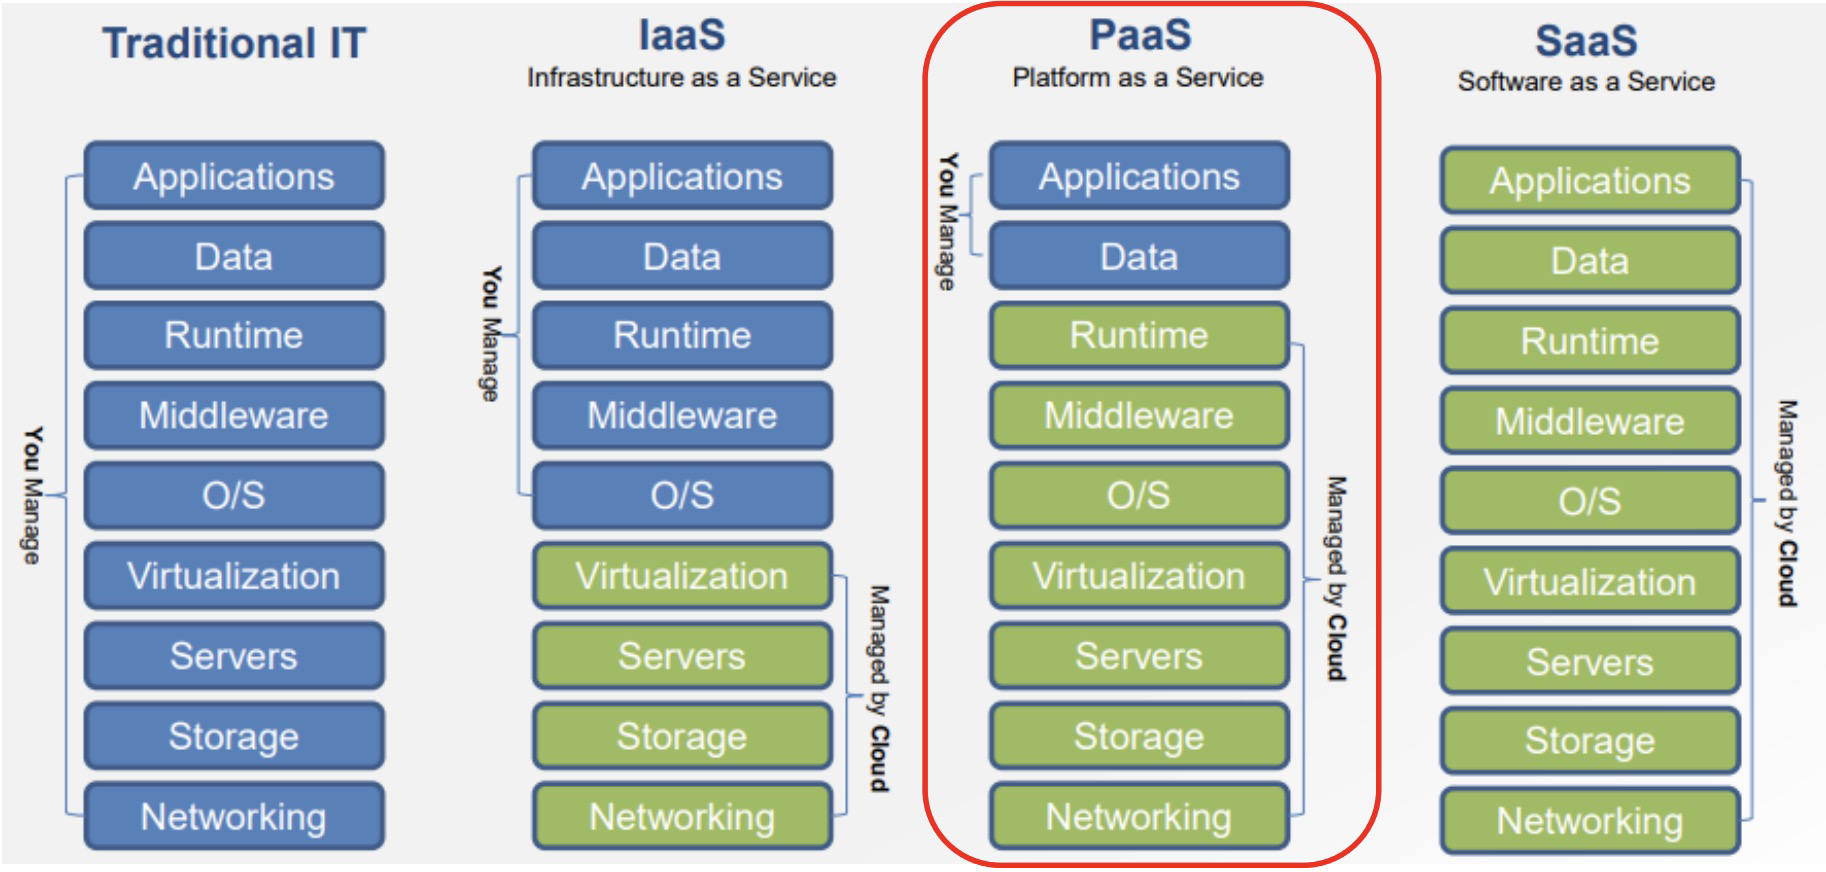
\includegraphics[width=0.7\textwidth]{14.png}
    \caption{Comparison: IaaS vs PaaS vs SaaS}
    % \label{fig:enter-label}
\end{figure}

\paragraph{Fetta di mercato} PaaS $<$ IaaS $<$ SaaS dovuto al fatto che l'utente target del PaaS è uno sviluppatore, mentre IaaS e SaaS sono rivolti ad un bacino di utenza molto più vasto.  Il PaaS attrae principalmente per l'aspetto di \textbf{application development}
\begin{figure}[h!]
    \centering
    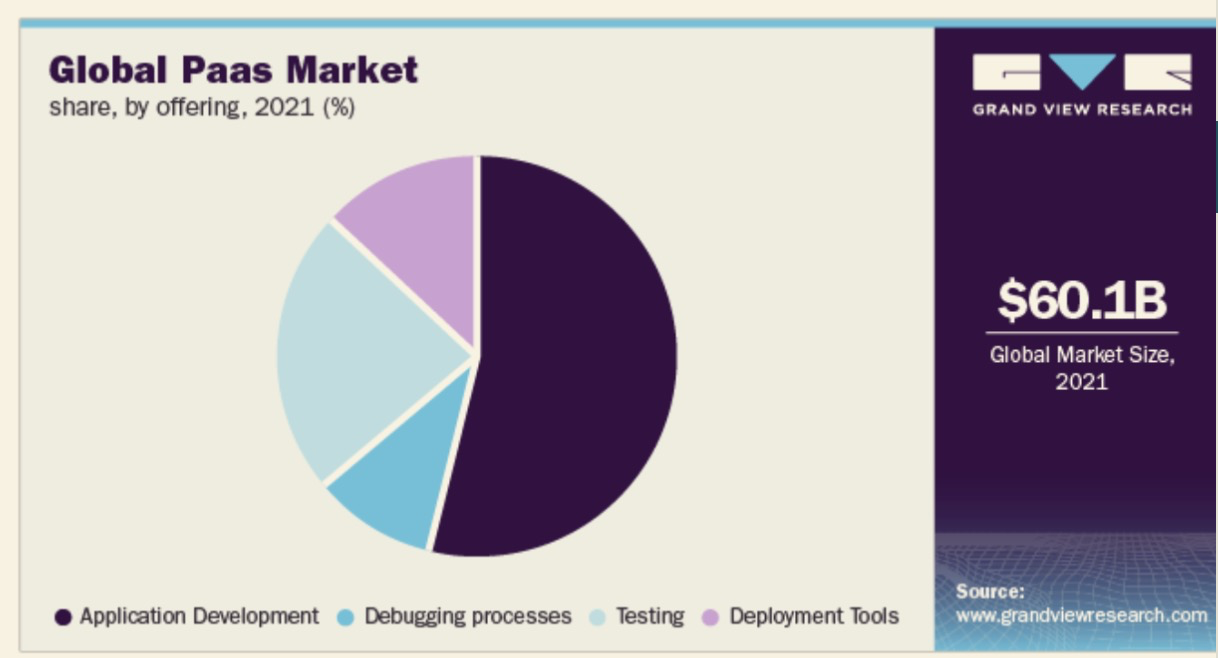
\includegraphics[width=0.7\textwidth]{15.png}
    \caption{Il servizio di PaaS più usato è quello di Application Development}
    % \label{fig:enter-label}
\end{figure}

\subsection{Heroku}
Heroku è una piattaforma Cloud che fornisce servizi integrati e un intero sistema che permette non solo di fare il deployment delle applicazioni, ma anche di modificarle, mandarle in esecuzione e gestirle.\\
Heroku nasce nel 2007 e viene acquisito da Salesforce nel 2010 per \$212M\\
I Container risolvono il grosso problema della \textbf{portabilità}: tramite Docker viene prelevata l’immagine del Container e ricostruita l’applicazione.  Heroku utilizza un sistema di Container chiamati \textbf{Dynos}, containers Linux virtualizzati che eseguono il codice fornito dall’utente: in pratica Heroku prende dall'utente un'applicazione non containerizzata e la incapscula in container.\\
I Dynos consentono una scalabilità molto flessibile, infatti a seconda delle richieste e delle risorse l’applicazione può scalare arbitrariamente il numero di Dynos.\\
Si può anche gestire il tipo, numero e dimensione di Dynos per applicazione, quindi l’utente non si deve preoccupare della gestione dell’infrastruttura e della scalabilità dell’applicazione.\\

\paragraph{Funzionamento} L'applicazione riceve la richiesta e la inoltra ad uno dei \textit{Web Dynos}; la richiesta viene analizzata e messa in coda asincrona (ottima per la scalabilità orizzontale); il \textit{Worker Dyno} gestisce la richiesta e la soddisfa, se è necessario può memorizzare in maniera persistente il risultato in un database. In questo caso la scalabilità permette di aumentare il numero di Web Dynos in modo da poter gestire un elevato numero di richieste contemporaneamente
\begin{figure}[h!]
    \centering
    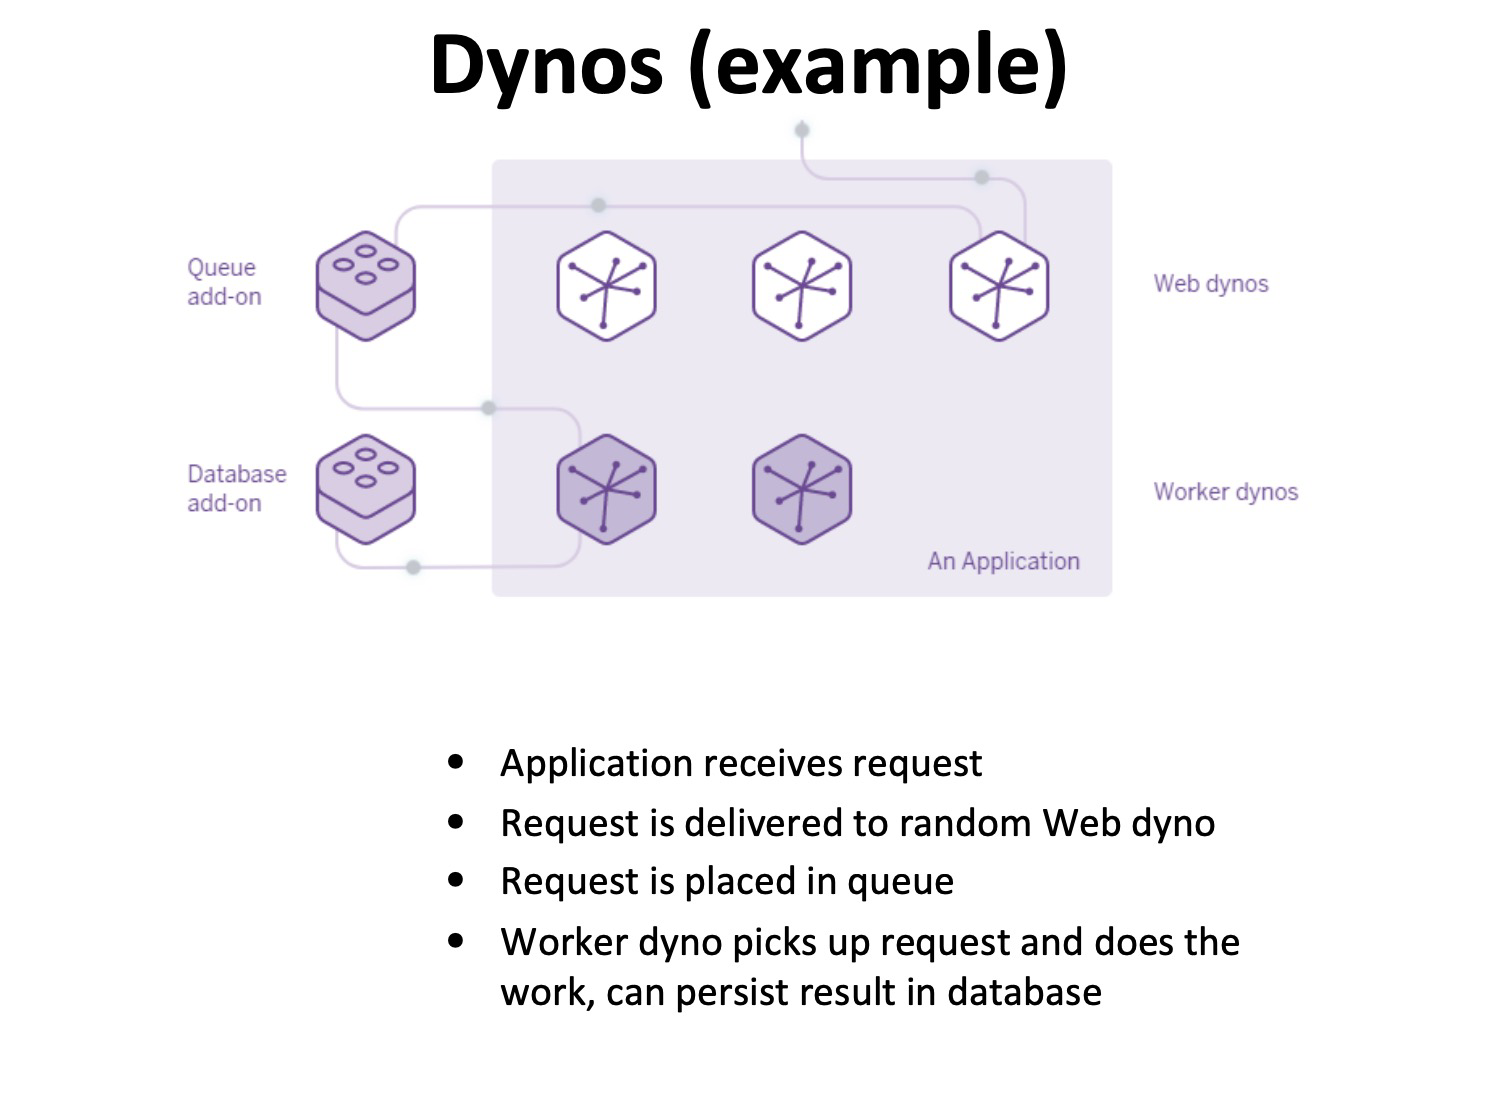
\includegraphics[width=0.7\textwidth]{16.png}
    \caption{Schema che rappresenta il funzionamento dei Dynos di Heroku}
    % \label{fig:enter-label}
\end{figure}

\subsubsection{Fasi Heroku}
\begin{enumerate}
    \item \textbf{Buildtime}: Heroku richiede tre componenti per costruire l'applicazione
    \begin{enumerate}
        \item codice sorgente
        \item lista di dipendenze
        \item un \textit{procfile},cioè un file di testo che contiene il comando per far partire il codice
    \end{enumerate}
    Una volta fornite queste tre cose, parte il sistema automatico di build: dopo aver ricevuto il codice, scarica il \textit{Build Packet} (linguaggio, dipendenze, librerie, ...), produce uno \textbf{slug} e lo mette in esecuzione in un Dynos. Il componente finale per eseguire l’applicazione è il sistema operativo (Ubuntu) che è aggiunto autonomamente da Heroku e si chiama \textbf{stack}

    \item \textbf{Runtime}: quando si fa il deployment o si scala manualmente l’applicazione, Heroku crea uno o più Dynos dove ognuno avrà lo stesso stack e slug che rappresenta un'istanza dell’applicazione.\\
    A questo punto Heroku esegue il comando che l’utente ha specificato nel \textit{procfile} per lanciare l’applicazione. Heroku permette di configurare le risorse che a tempo di esecuzione si vogliono utilizzare, per esempio esistono quattro tipi principali di Dynos:
    \begin{enumerate}
        \item \textit{free/hobby}, che comprendono le funzionalità di base
        \item \textit{standard}, che supportano la scalabilità orizzontale
        \item \textit{performance}, che oltre alla scalabilità orizzontale supporta anche l'\textbf{autoscaling} in cui si stabilisce a priori secondo quali parametri Heroku dovrà scalare
    \end{enumerate}

    \item \textbf{Add-ons}: Heroku ha 150+ add-ons che gli sviluppatori possono utilizzare per estendere le funzionalità dell’applicazione.\\
    Per esempio servizio di autenticazione, logging, monitoring, data stores... Tutto questo attrae l’utente perché può integrare rapidamente nuove features senza doverle costruire lui stesso from scratch.\\
    L’aspetto negativo è che l'utente è legato all’utilizzo della piattaforma e instaura una forma di \textbf{vendor lock-in} rendendo la nostra applicazione più difficilmente portabile. Infatti se volessimo spostare la nostra applicazione su un nuovo servizio Cloud saremo costretti a rivedere tutto il codice perché gli add-ons non sarebbero più disponibili
\end{enumerate}

\begin{figure}[h!]
    \centering
    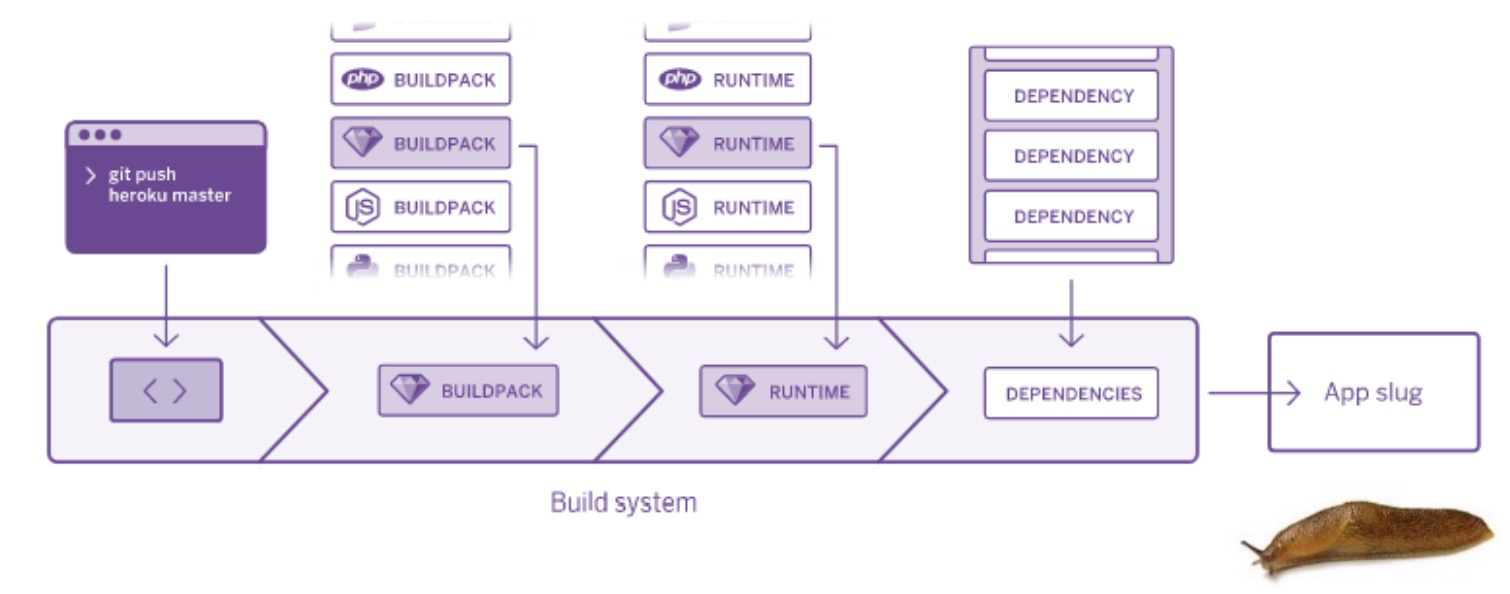
\includegraphics[width=0.7\textwidth]{17.png}
    \caption{Schema che rappresenta le fasi di Heroku per produrre l'app slug}
    % \label{fig:enter-label}
\end{figure}

\subsection{\href{https://www.youtube.com/watch?v=0d1OO79brYY}{Microsoft Azure}}
Microsoft Azure offre funzionalità simili a Heroku tra cui:
\begin{itemize}
    \item scalabilità verticale
    \item supporto di diversi linguaggi
    \item strumenti per sviluppatori (developer tools)
    \item SQL database
    \item meccanismi di sicurezza
    \item data storage
    \item machine learning per analisi predittive
    \item servizi media per supportare video.
\end{itemize}
Azure, che viene presentato come PaaS, è in realtà un \textit{IaaS+PaaS} perché la API che fornisce è molto ricca di funzionalità 

\subsection{\href{https://www.youtube.com/watch?v=XfTRyF6TX6o&list=PLaR6Rq6Z4Iqficb-XqeydZD_ZTD3XEwBp}{OpenShift}}
Red Hat OpenShift è una piattaforma PaaS molto utilizzata. Ci sono molte funzionalità semplici per il build e il deployment automatico. OpenShift è basato su Kubernetes (si veda capitolo \ref{container}) e può monitorare lo stato delle applicazioni facendole ripartire automaticamente in caso di fallimenti.\\
E` una piattaforma DevOps che permette la costruzione e l’erogazione dei servizi, infatti con OpenShift un'organizzazione può costruire il proprio workflow DevOps cioè un modo di lavorare che permette ai team di collaborare mantenendo autonomia.
\paragraph{Consigliato} \href{https://www.youtube.com/watch?v=IO_uap5wfUU}{OpenShift for Beginners - demo voting app}

\subsection{Google Firebase}
Firebase è il PaaS di Google, successore del primo PaaS che presentò (ai tempi chiamato \textit{GAE}). Il prossimo laboratorio sarà dedicato ad un \textit{hands-on} su Google Firebase. (si veda capitolo \ref{lab4})